\documentclass{article}

\usepackage{amsmath,amsthm,amssymb}
\usepackage{commath}
\usepackage{mathtools}
\usepackage{enumerate}
\usepackage{subcaption}
\usepackage{float}
\usepackage{tikz}
\usepackage[margin=1in]{geometry}

\usetikzlibrary{positioning}

\setlength{\parindent}{0pt}
\setlength{\parskip}{8pt}

\usepackage[utf8]{inputenc}
\begin{document}
\title{Assignment 6 \\ Advanced Algorithms \& Data Structures PS}%
\author{Christian Müller 1123410 \\ Daniel Kocher, 0926293}%
\maketitle

{\bfseries Aufgabe 11}%
{\parskip0pt
  \begin{enumerate}[i.)]
  \item F{\"u}gen Sie die Schl{\"u}ssel $f$, $g$, $h$, $e$, $b$, $a$, $c$ in einen
    (anfangs leeren) Treap ein. Die Priorit{\"a}ten dieser Schl{\"u}ssel sind
    wie folgt gegeben: $a:8$, $b:15$, $c:2$, $e:3$, $f:7$, $g:6$, $h:25$, $i:22$,
    $j:19$, $k:13$.
  \item Entfernen Sie $e$ aus dem Treap.
  \item F{\"u}gen Sie die Schl{\"u}ssel $i$, $j$, $k$ in einen anderen (anfangs
    leeren) Treap ein. Vereinigen Sie anschlie{\ss}end die zwei Treaps.
  \item F{\"u}hren Sie $Spalte \left( T, d, T_1, T_2 \right)$ durch, wobei $T$
    der Treap aus dem vorigen Punkt ist.
  \end{enumerate}
}
Geben Sie den Treap vor und nach jeder Rotation an.

\medskip%

F{\"u}r den Pseudocode bzw. die grundlegenden Vorgehensweise der Operationen
Suchen, Einf{\"u}gen, RotiereNachLinks/Rechts, Entfernen, Vereinige und Spalte,
sei auf die Folien vom 14.04.2016 verwiesen.

%\clearpage
i.)

\begin{figure}[H]
  \centering
  \begin{subfigure}[b]{.4\textwidth}
    \centering
    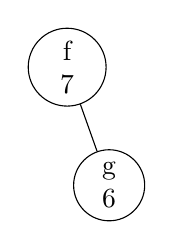
\begin{tikzpicture}[every node/.style = { draw, align = center, shape = circle }]
      \node { f \\ 7 }
      child { node [right = .75mm] { g \\ 6 } };
    \end{tikzpicture}
    \label{subfig:aufg9-i-1-before}
    \caption{Vorher}
  \end{subfigure}
  \quad
  \begin{subfigure}[b]{.4\textwidth}
    \centering
    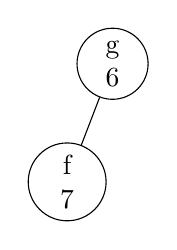
\begin{tikzpicture}[every node/.style = { draw, align = center, shape = circle }]
      \node { g \\ 6 }
      child { node [left = .75mm] { f \\ 7 } };
    \end{tikzpicture}
    \label{subfig:aufg9-i-1-after}
    \caption{Nachher}
  \end{subfigure}
  \label{fig:aufg9-i-1}
  \caption{1. Rotation: nach links (1x) (nach Einf{\"u}gen von $f$, $g$)}
\end{figure}

\begin{figure}[H]
  \centering
  \begin{subfigure}[b]{.4\textwidth}
    \centering
    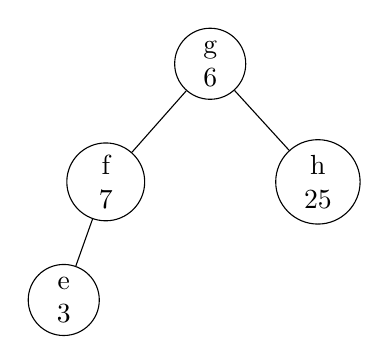
\begin{tikzpicture}[every node/.style = { draw, align = center, shape = circle }]
      \node { g \\ 6 }
      child { node [left = .75mm] { f \\ 7 } 
        child { node [left = .75mm] { e \\ 3 } }
      }
      child { node [right = .75mm] { h \\ 25 } };
    \end{tikzpicture}
    \label{subfig:aufg9-i-1-before}
    \caption{Vorher}
  \end{subfigure}
  \quad
  \begin{subfigure}[b]{.4\textwidth}
    \centering
    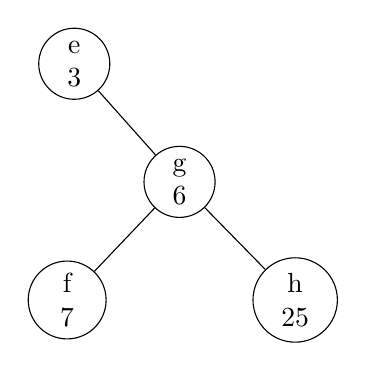
\begin{tikzpicture}[every node/.style = { draw, align = center, shape = circle }]
      \node { e \\ 3 }
      child { node [right = 2.5em] { g \\ 6  } 
        child { node [left = .5em] { f \\ 7 } }
        child { node [right = .5em] { h \\ 25 } } 
      };
    \end{tikzpicture}
    \label{subfig:aufg9-i-1-after}
    \caption{Nachher}
  \end{subfigure}
  \label{fig:aufg9-i-1}
  \caption{2. Rotation: nach rechts (2x) (nach Einf{\"u}gen von $h$, $e$)}
\end{figure}

\begin{figure}[H]
  \centering
  \begin{subfigure}[b]{.45\textwidth}
    \centering
    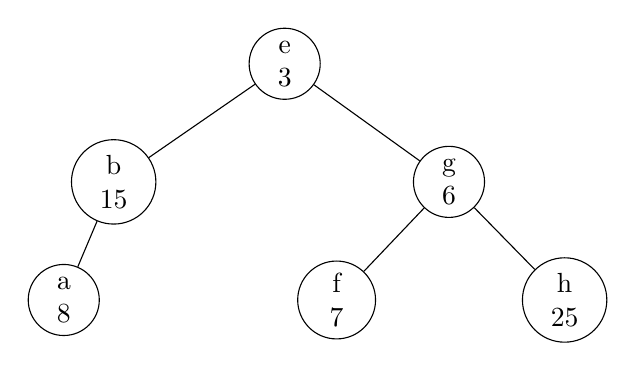
\begin{tikzpicture}[every node/.style = { draw, align = center, shape = circle }]
      \node { e \\ 3 }
      child { node [left = 2.5em] { b \\ 15 }
        child { node [left = .5em] { a \\ 8 } }
      }
      child { node [right = 2.5em] { g \\ 6  } 
        child { node [left = .5em] { f \\ 7 } }
        child { node [right = .5em] { h \\ 25 } } 
      };
    \end{tikzpicture}
    \label{subfig:aufg9-i-1-before}
    \caption{Vorher}
  \end{subfigure}
  \quad
  \begin{subfigure}[b]{.45\textwidth}
    \centering
    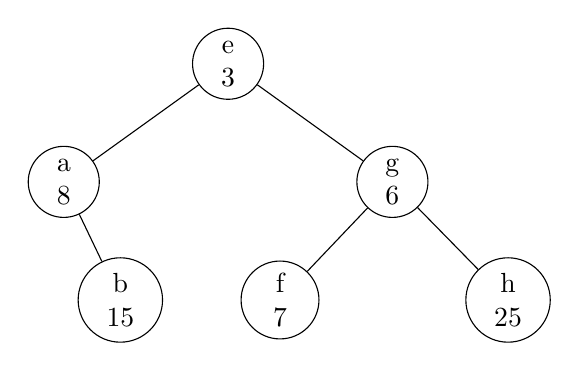
\begin{tikzpicture}[every node/.style = { draw, align = center, shape = circle }]
      \node { e \\ 3 }
      child { node [left = 2.5em] { a \\ 8 }
        child { node [right = .5em] { b \\ 15 } }
      }
      child { node [right = 2.5em] { g \\ 6  } 
        child { node [left = .5em] { f \\ 7 } }
        child { node [right = .5em] { h \\ 25 } } 
      };
    \end{tikzpicture}
    \label{subfig:aufg9-i-1-after}
    \caption{Nachher}
  \end{subfigure}
  \label{fig:aufg9-i-1}
  \caption{3. Rotation: nach rechts (1x) (nach Einf{\"u}gen von $b$, $a$)}
\end{figure}

\begin{figure}[H]
  \centering
  \begin{subfigure}[b]{.45\textwidth}
    \centering
    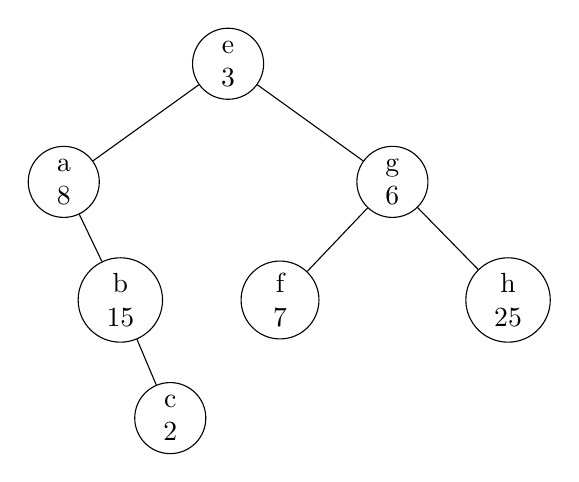
\begin{tikzpicture}[every node/.style = { draw, align = center, shape = circle }]
      \node { e \\ 3 }
      child { node [left = 2.5em] { a \\ 8 }
        child { node [right = .5em] { b \\ 15 } 
          child { node [right = .5em] { c \\ 2 } }
        }
      }
      child { node [right = 2.5em] { g \\ 6  } 
        child { node [left = .5em] { f \\ 7 } }
        child { node [right = .5em] { h \\ 25 } } 
      };
    \end{tikzpicture}
    \label{subfig:aufg9-i-1-before}
    \caption{Vorher}
  \end{subfigure}
  \quad
  \begin{subfigure}[b]{.45\textwidth}
    \centering
    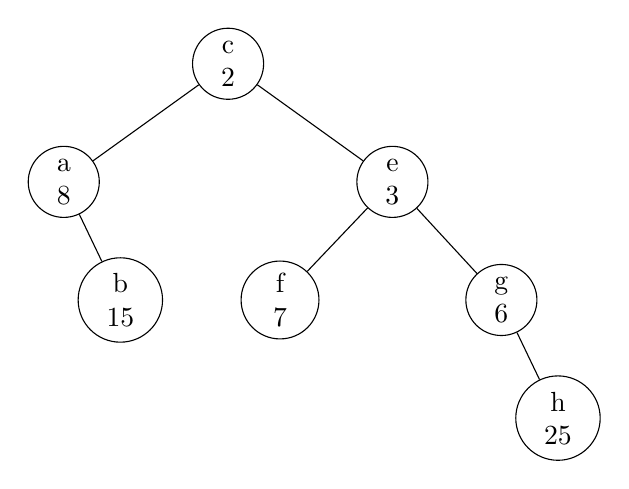
\begin{tikzpicture}[every node/.style = { draw, align = center, shape = circle }]
      \node { c \\ 2 }
      child { node [left = 2.5em] { a \\ 8 }
        child { node [right = .5em] { b \\ 15 } }
      }
      child { node [right = 2.5em] { e \\ 3  } 
        child { node [left = .5em] { f \\ 7 } }
        child { node [right = .5em] { g \\ 6 }
          child { node [right = .5em] { h \\ 25 } }
        }
      };
    \end{tikzpicture}
    \label{subfig:aufg9-i-1-after}
    \caption{Nachher}
  \end{subfigure}
  \label{fig:aufg9-i-1}
  \caption{4. Rotation: nach links (2x), nach rechts (1x) (nach Einf{\"u}gen von $c$)}
\end{figure}

{\bfseries Aufgabe 12}%

Der {\it linke Rand} in einem bin{\"a}ren Suchbaum $T$ ist der Pfad von der Wurzel
zum Knoten mit dem kleinsten Schl{\"u}ssel. Der {\it rechte Rand} in einem
bin{\"a}ren Suchbaum $T$ ist der Pfad von der Wurzel zum Knoten mit dem
gr{\"o}{\ss}ten Schl{\"u}ssel. Betrachten Sie einen Treap $T$ direkt nach dem
Einf{\"u}gen eines Objektes $x$. Sei $C$ die L{\"a}nge des rechten Randes des
linken Unterbaums des Knotens mit dem Element $x$ und sei $D$ die L{\"a}nge des
linken Randes des rechten Unterbaums des Knotens mit dem Element $x$. Zeigen Sie,
dass die Anzahl der Rotationen, die w{\"a}hrend des Einf{\"u}gens von $x$
durchgef{\"u}hrt wurden, $C + D$ ist.

\medskip%

{\bfseries Aufgabe 13}%

Sei $U = \left\{ 0, \ldots, N - 1 \right\}$, wobei $N$ eine Primzahl ist und sei
$m = 4$. Seien $a_i = 40i$ und $b_i = 60i$. Wir definieren folgende Klasse von
Hashfunktionen:
\begin{equation}
  H = \left\{ h_i \left( k \right) = \left( \left( a_ik + b_i \right)\text{ mod }N - 1 \right)\text{ mod }m \right\}
  \text{ f{\"u}r } i \in \left\{ 1, \ldots, N \left( N - 1 \right) \right\}
\end{equation}
Ist $H$ universell? Warum? Falls $H$ nicht universell ist, so modifizieren Sie
$h_i$, $a_i$ und $b_i$, sodass Sie eine universelle Klasse erhalten.

\medskip%\\

\end{document}
